\documentclass[headinclude,DIV12]{scrartcl}

\usepackage[latin1]{inputenc}
\usepackage[T1]{fontenc}
\usepackage[english]{babel}

\usepackage{scrpage2}
\usepackage{url}
%
\usepackage{pst-optexp}
\let\verPstOptExp\fileversion
\let\datePstOptExp\filedate
\usepackage{multicol}
\usepackage{showexpl}
\lstset{breakatwhitespace}
\usepackage{nicefrac}
\usepackage{graphicx}
\usepackage[colorlinks,linktocpage]{hyperref}
\usepackage{xspace}
%
% New commands
%
\DeclareRobustCommand\cs[1]{\texttt{\char`\\#1}}
\newcommand{\OptExpPackage}{\textsf{`pst-optexp'}}
\newcommand{\parameter}[1]{\texttt{#1}}
\let\param\textrm
\newcommand{\defaultparam}{\emph{default:}\xspace}

%
% Settings
\setkomafont{sectioning}{\normalfont\normalcolor\bfseries}
%
\makeatletter
\renewenvironment{description}
  {\list{}{\labelwidth\z@ \itemindent-\leftmargin
    \itemsep0pt \parsep0pt
    \let\makelabel\descriptionlabel}}
  {\endlist}
\makeatother
%
\clearscrheadfoot
\setheadsepline{0.4pt}
\ihead{\OptExpPackage}\ohead{A PSTricks package to draw optical experimental setups}
\pagestyle{scrheadings}

\psset{subgriddiv=0,griddots=10,gridlabels=7pt}

%%%%%%%%%%%%%%%%%%%%%%%%%%%%%%%%%%%%%%%%%%%%%%%%%%%%%%%%%%%%%%%%%%%%%%%%
\begin{document}
 \title{\texttt{pst-optexp}\\ A PSTricks package to draw optical experimental setups}
 \author{Christoph Bersch \textless
   \href{mailto:usenet@bersch.net}{\texttt{usenet@bersch.net}}\textgreater}
 \date{\datePstOptExp\enspace\enspace Version \verPstOptExp}

\maketitle

\setlength{\columnseprule}{0.6pt}
\begin{multicols}{2}
{\parskip 0pt \tableofcontents}
\end{multicols}
\section{Introduction}
The package \texttt{pst-optexp} is a collection of optical components
that facilitate easy sketching of optical experimental
setups. Mechanisms for proper alignment of different components are
provided internally. This way the user does not have to care for proper
orientation of the elements. Macros for using user-defined components
are also provided.

\section{Components}

In the sections \ref{sec:lens}--\ref{sec:custom} the
available components with their parameters are described. Up to now
there are two types of components: those which require two reference
points and do not alter the direction of the passing light beam (for
example lenses and retardation plates) and those which work in
reflection and require three reference points (mirrors, grids,
beamsplitters etc.).

In section \ref{sec:general} general parameters are described that are
not proprietary to a specific unit but can be used for several different
components. Finally, in section \ref{sec:labels} the options for the
positioning of labels are explained.

The appearence of all components can be changed with the corresponding
standard PSTricks parameters such as \parameter{fillstyle}
or \parameter{linestyle}. For some components changing only parts of the
layout may be desired (e.g. the extended part of mirrors). For those
cases psstyles are provided that influence only the corresponing part of the
components and can be redefined using \cs{newpsstyle}.

\subsection{Lens}\label{sec:lens}

\begin{description}
\item[\param{lensheight} (dimension):] (\defaultparam 1)
\item[\param{lenswidth} (dimension):] (\defaultparam 0.3)
\item[\param{lensradius} (dimension):] (\defaultparam \texttt{\cs{empty}})
\item[\param{lenstype} (plainconvex\,|\,plainconcave\,|\,convexplain\,|\,concaveplain\,|\,biconvex\,|\,biconcave):]~\\
  (\defaultparam \texttt{biconvex})
\end{description}

For the convex lenses only two parameters are used. If the
parameter \parameter{lensradius} is set, its value will be used together
with \parameter{lensheight} to draw the
lens. Otherwise \parameter{lenswidth} and
\parameter{lensheight} are used. For concave lenses all three parameters
are required.

\medskip

\begin{LTXexample}[width=3.5cm]
\begin{pspicture}(3,2)\psgrid
  \pnode(0,1.8){A}
  \pnode(3,0.7){B}
  \psline[linecolor=green](A)(B)
  \lens[lenstype=plainconvex](A)(B){lens}
\end{pspicture}
\end{LTXexample}

\bigskip

\begin{LTXexample}[width=3.5cm]
\begin{pspicture}(3,2)\psgrid
  \pnode(0,1.8){A}
  \pnode(3,0.7){B}
  \psline[linecolor=green](A)(B)
  \lens[lenstype=convexplain](A)(B){lens}
\end{pspicture}
\end{LTXexample}

\bigskip

\begin{LTXexample}[width=3.5cm]
\begin{pspicture}(3,2)\psgrid
  \pnode(0,1.8){A}
  \pnode(3,0.7){B}
  \psline[linecolor=green](A)(B)
  \lens(A)(B){lens}
\end{pspicture}
\end{LTXexample}

\bigskip
\begin{LTXexample}[width=3.5cm]
\begin{pspicture}(3,2)\psgrid
  \pnode(0,1.8){A}
  \pnode(3,0.7){B}
  \psline[linecolor=green](A)(B)
  \lens[lenstype=plainconcave](A)(B){lens}
\end{pspicture}
\end{LTXexample}

\bigskip
\begin{LTXexample}[width=3.5cm]
\begin{pspicture}(3,2)\psgrid
  \pnode(0,1.8){A}
  \pnode(3,0.7){B}
  \psline[linecolor=green](A)(B)
  \lens[lenstype=concaveplain](A)(B){lens}
\end{pspicture}
\end{LTXexample}

\bigskip
\begin{LTXexample}[width=3.5cm]
\begin{pspicture}(3,2)\psgrid
  \definecolor{lensColor}{rgb}{0.7, 0.9, 1}
  \pnode(0,1.8){A}
  \pnode(3,0.7){B}
  \psline[linecolor=green](A)(B)
  \lens[lenstype=biconcave,
        fillstyle=solid,
        fillcolor=lensColor](A)(B){lens}
\end{pspicture}
\end{LTXexample}

\medskip

\subsection{Optical plate}

\begin{description}
\item[\param{plateheight} (dimension):] (\defaultparam 1)
\item[\param{platelinewidth} (dimension):] (\defaultparam 2\cs{pslinewidth})
\end{description}

\medskip

\begin{LTXexample}[width=3.5cm]
\begin{pspicture}(3,2)\psgrid
  \pnode(0,1.2){A}
  \pnode(3,1.2){B}
  \psline[linecolor=green](A)(B)
  \optplate(A)(B){filter}
\end{pspicture}
\end{LTXexample}

\medskip

\subsection{Retardation plate}

\begin{description}
\item[\param{plateheight} (dimension):] (\defaultparam 1)
\item[\param{platewidth} (dimension):] (\defaultparam 0.1)
\end{description}

\medskip

\begin{LTXexample}[width=3.5cm]
\begin{pspicture}(3,2)\psgrid
  \pnode(0,1.2){A}
  \pnode(3,1.2){B}
  \psline[linecolor=green](A)(B)
  \optretplate(A)(B){$\nicefrac{\lambda}{2}$}
\end{pspicture}
\end{LTXexample}

\medskip

\subsection{Pinhole}

\begin{description}
\item[\param{outerheight} (dimension):] (\defaultparam 1)
\item[\param{innerheight} (dimension):] (\defaultparam 0.1)
\item[\param{phlinewidth} (dimension):]  (\defaultparam 2\cs{pslinewidth})
\end{description}

\medskip

\begin{LTXexample}[width=3.5cm]
\begin{pspicture}(3,2)\psgrid
  \pnode(0,1.2){A}
  \pnode(3,1.2){B}
  \psline[linecolor=green](A)(B)
  \pinhole(A)(B){PH}
\end{pspicture}
\end{LTXexample}

\medskip

\subsection{Crystal}

\begin{description}
\item[\param{crystalwidth} (dimension):] (\defaultparam 2)
\item[\param{crystalheight} (dimension):] (\defaultparam 0.8)
\item[\param{caxislength} (dimension):] (\defaultparam 0.6)
\item[\param{caxisinv} (boolean):] (\defaultparam \texttt{false})
\item[\param{voltage} (boolean):] (\defaultparam \texttt{false})
\item[\param{lamp} (boolean):] (\defaultparam \texttt{false})
\item[\param{lampscale} (real):] (\defaultparam 0.3)
\end{description}

\medskip

\begin{LTXexample}[width=3.5cm]
\begin{pspicture}(3,2)\psgrid
  \pnode(0,1.2){A}
  \pnode(3,1.2){B}
  \crystal[crystalwidth=1.5,
           crystalheight=0.6,
           fillstyle=solid,
           fillcolor=yellow!90!black,
           labelangle=-45,
           labeloffset=1.2,
           voltage,
           lamp](A)(B){SBN:Ce}
  \psline[linecolor=green](A)(B)
\end{pspicture}
\end{LTXexample}

\medskip

\subsection{Box}

\begin{description}
\item[\param{optboxheight} (dimension):] (\defaultparam 0.5)
\item[\param{optboxwidth} (dimension):] (\defaultparam 1)
\item[\param{endbox} (boolean):] (\defaultparam \texttt{false})
\end{description}

\medskip 

\begin{LTXexample}[width=3.5cm]
\begin{pspicture}(3,2)\psgrid
  \pnode(0,0){A}
  \pnode(3,2){B}
  \psline[linecolor=green](A)(B)
  \optbox(A)(B){box}
\end{pspicture}
\end{LTXexample}

\bigskip

\begin{LTXexample}[width=3.5cm]
\begin{pspicture}(3,2)\psgrid
  \pnode(0,0){A}
  \pnode(1.7,1){B}
  \psline[linecolor=green](A)(B)
  \optbox[endbox](A)(B){box}
\end{pspicture}
\end{LTXexample}

\bigskip

\begin{LTXexample}[width=3.5cm]
\begin{pspicture}(3,2)\psgrid
  \pnode(0,0){A}
  \pnode(1.7,1){B}
  \psline[linecolor=green](A)(B)
  \optbox[endbox,labelref=relative,labeloffset=0](A)(B){box}
\end{pspicture}
\end{LTXexample}

\medskip

\subsection{Detector}

\begin{description}
\item[\param{detsize} (dimension):] (\defaultparam 0.5)
\end{description}

\medskip 

\begin{LTXexample}[width=3.5cm]
\begin{pspicture}(3,2)\psgrid
  \pnode(0,0){A}
  \pnode(1.7,1){B}
  \psline[linecolor=green](A)(B)
  \detector(A)(B){detector}
\end{pspicture}
\end{LTXexample}

\medskip

\subsection{Polarization}

\begin{description}
\item[\param{poltype} (parallel | perp | misc | lcirc | rcirc):] (\defaultparam \texttt{parallel})
\item[\param{polsize} (dimension):] (\defaultparam 0.6)
\item[\param{pollinewidth} (dimension):] (\defaultparam 0.7\cs{pslinewidth})
\end{description}

\medskip

\begin{LTXexample}[width=3.4cm]
\begin{pspicture}(3,5)\psgrid
  \pnode(0,0.5){A1}\pnode(3,0.5){B1}\pnode(0,1.5){A2}
  \pnode(3,1.5){B2}\pnode(0,2.5){A3}\pnode(3,2.5){B3}
  \pnode(0,3.5){A4}\pnode(3,3.5){B4}\pnode(0,4.5){A5}
  \pnode(3,4.5){B5}\psset{linecolor=green}
  \multido{\i=1+1}{5}{\psline(A\i)(B\i)}
  \psset{linecolor=black}
  \polarization[poltype=misc,position=0.2](A5)(B5)
  \polarization[poltype=perp,position=0.35](A4)(B4)
  \polarization[poltype=parallel,position=0.5](A3)(B3)
  \polarization[poltype=rcirc,position=0.65](A2)(B2)
  \polarization[poltype=lcirc,position=0.8](A1)(B1)
\end{pspicture}
\end{LTXexample}

\medskip

\subsection{Mirror}\label{sec:mirror}

\begin{description}
\item[\param{mirrorwidth} (dimension):] (\defaultparam 1)
\item[\param{mirrorlinewidth} (dimension):] (\defaultparam 2\cs{pslinewidth})
\item[\param{mirrortype} (normal | piezo | extended):] (\defaultparam \texttt{normal})
\item[\param{mirrordepth} (dimension):] (\defaultparam 0.08)
\item[\param{variable} (boolean):] (\defaultparam \texttt{false})
\end{description}

The style of the extended mirror is defined as a
psstyle \parameter{ExtendedMirror} and can be changed using
\cs{newpsstyle}. The appearence of the piezo mirror likewise can be
changed by adapting the psstyle \parameter{PiezoMirror}.

\medskip

\begin{LTXexample}[width=3.5cm]
\begin{pspicture}(3,3)\psgrid
  \pnode(0,0){A}
  \pnode(1.8,2.2){G}
  \pnode(0,3){B}
  \psline[linecolor=green](A)(G)(B)
  \mirror(A)(G)(B){mirror}
\end{pspicture}
\end{LTXexample}

\bigskip

\begin{LTXexample}[width=3.5cm]
\begin{pspicture}(3,3)\psgrid
  \pnode(0,0){A}
  \pnode(1.8,2.2){G}
  \pnode(0,3){B}
  \psline[linecolor=green](A)(G)(B)
  \mirror[variable](A)(G)(B){M$_\mathrm{var}$}
\end{pspicture}
\end{LTXexample}

\bigskip

\begin{LTXexample}[width=3.5cm]
\begin{pspicture}(3,3)\psgrid
  \pnode(0,0){A}
  \pnode(1.8,2.2){G}
  \pnode(0,3){B}
  \psline[linecolor=green](A)(G)(B)
  \mirror[mirrortype=piezo,labelangle=-90](A)(G)(B){piezo}
\end{pspicture}
\end{LTXexample}

\bigskip

\begin{LTXexample}[width=3.5cm]
\begin{pspicture}(3,3)\psgrid
  \pnode(0,0){A}
  \pnode(1.8,2.2){G}
  \pnode(0,3){B}
  \psline[linecolor=green](A)(G)(B)
  \mirror[mirrortype=extended](A)(G)(B){M$_\mathrm{ext}$}
\end{pspicture}
\end{LTXexample}

\medskip

\subsection{Beamsplitter}

\begin{description}
\item[\param{bssize} (dimension):] (\defaultparam 0.8)
\end{description}

\medskip

\begin{LTXexample}[width=3.5cm]
\begin{pspicture}(3,3)\psgrid
  \pnode(0,2){A}
  \pnode(2,2){G}
  \pnode(3,0){B}
  \psline[linecolor=green](A)(G)(B)
  \beamsplitter(A)(G)(B){BS}
\end{pspicture}
\end{LTXexample}

\medskip


\subsection{Optical grid}

\begin{description}
\item[\param{optgridcount} (integer):] (\defaultparam 10)
\item[\param{optgridwidth} (dimension):] (\defaultparam 1)
\item[\param{optgridheight} (dimension):] (\defaultparam 0.1)
\item[\param{optgriddepth} (dimension):] (\defaultparam 0.05)
\item[\param{optgridlinewidth} (dimension):] (\defaultparam 0.7\cs{pslinewidth})
\item[\param{reverse} (boolean):] (\defaultparam \texttt{false})
\end{description}

\medskip

\begin{LTXexample}[width=3.5cm]
\begin{pspicture}(3,3)\psgrid
  \pnode(0,3){A}
  \pnode(1.8,2.2){G}
  \pnode(0,0){B}
  \psline[linecolor=green](A)(G)(B)
  \optgrid(A)(G)(B){grid}
\end{pspicture}
\end{LTXexample}

\bigskip


\begin{LTXexample}[width=3.5cm]
\begin{pspicture}(3,3)\psgrid
  \pnode(0,3){A}
  \pnode(1.8,2.2){G}
  \pnode(0,0){B}
  \psline[linecolor=green](A)(G)(B)
  \optgrid[reverse](A)(G)(B){grid}
\end{pspicture}
\end{LTXexample}

\bigskip

\begin{LTXexample}[width=3.5cm]
\begin{pspicture}(3,3)\psgrid
  \pnode(0,3){A}
  \pnode(1.8,2.2){G}
  \pnode(0,0){B}
  \psline[linecolor=green](A)(G)(B)
  \optgrid[optgridcount=6,%
           optgriddepth=0.2,%
           optgridheight=0.3](A)(G)(B){grid}
\end{pspicture}
\end{LTXexample}

\medskip

\subsection{Custom components}\label{sec:custom}

\begin{LTXexample}[width=3.5cm]
\begin{pspicture}(3,3)\psgrid
  \pnode(0,2){A}
  \pnode(3,1){B}
  \optdipole[labeloffset=1](A)(B){%
    \rput(0,0){%
      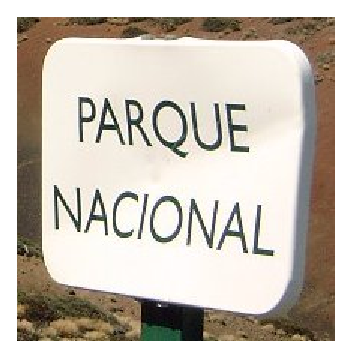
\includegraphics[scale=0.25]{parque-nacional}
    }
  }{label}
  \psline[linecolor=red](A)(B)
\end{pspicture}
\end{LTXexample}

\bigskip

\begin{LTXexample}[width=3.5cm]
\begin{pspicture}(3,3)\psgrid
  \pnode(0,0){A}
  \pnode(1.5,2){G}
  \pnode(3,1.5){B}
  \opttripole(B)(G)(A){\rput[b](0,0){text}}{label}
  \psline[linecolor=red](A)(G)(B)
\end{pspicture}
\end{LTXexample}

\medskip

\subsection{General options}\label{sec:general}

\begin{description}
\item[\param{angle} (real):] (\defaultparam 0)
\item[\param{optional} (boolean):] (\defaultparam \texttt{false})
\item[\param{position} (real):] (\defaultparam \texttt{\cs{empty}})
\item[\param{abspos} (dimension):] (\defaultparam \texttt{\cs{empty}})
\item[\param{showoptdots} (boolean):] (\defaultparam \texttt{false})
\end{description}

The parameter \parameter{angle} is available for the macros \cs{optbox}
and \cs{crystal} only, as for the most other cases it would make
no sense. \parameter{optional} can be used with every component and marks it as
optional and can be configured by changing the psstyle \parameter{OptionalStyle}.
\parameter{position} is equivalent to the \parameter{npos} parameter of \cs{ncput},
but is used only for the \lq dipole\rq-macros to position the component
between the two given points. In addition, there is a parameter
\parameter{abspos} that allows absolute positioning between the two line
points. \parameter{showoptdots} shows in black the two points calculated for the
positioning of the component, and in red the reference points for the
label.

\medskip

\begin{LTXexample}[width=3.5cm]
  \begin{pspicture}(3,2)\psgrid
    \pnode(0,1.2){A}
    \pnode(3,1.2){B}
    \psline[linecolor=green](A)(B)
    \optbox[angle=10](A)(B){box}
  \end{pspicture}
\end{LTXexample}

\bigskip

\begin{LTXexample}[width=3.5cm]
  \begin{pspicture}(3,2)\psgrid 
    \pnode(0,1.2){A} 
    \pnode(3,1.2){B}
    \psline[linecolor=green](A)(B) 
    \lens[optional](A)(B){L}
  \end{pspicture}
\end{LTXexample}

\bigskip

\begin{LTXexample}[width=3.5cm]
  \begin{pspicture}(3,2)\psgrid 
    \pnode(0,1.2){A} 
    \pnode(3,1.2){B}
    \psline[linecolor=green](A)(B) 
    \lens[position=0.8](A)(B){L}
  \end{pspicture}
\end{LTXexample}

\bigskip

\begin{LTXexample}[width=3.5cm]
  \begin{pspicture}(3,2)\psgrid 
    \pnode(0,1.2){A} 
    \pnode(3,1.2){B}
    \psline[linecolor=green](A)(B) 
    \lens[abspos=1](A)(B){L}
  \end{pspicture}
\end{LTXexample}

\bigskip

\begin{LTXexample}[width=3.5cm]
  \begin{pspicture}(3,3)\psgrid 
    \pnode(0,0){A} 
    \pnode(1.5,2){G}
    \pnode(0,3){B} 
    \psline[linecolor=green](A)(G)(B)
    \mirror[showoptdots](A)(G)(B){mirror}
  \end{pspicture}
\end{LTXexample}

\medskip

\subsection{Labels}\label{sec:labels}

\begin{description}
\item[\param{labeloffset} (dimension):] (\defaultparam 1)
\item[\param{labelangle} (real):] (\defaultparam 0)
\item[\param{labelstyle} (macro):] (\defaultparam \texttt{\cs{small}})
\item[\param{labelalign} (\cs{rput} ref string):] (\defaultparam \texttt{c})
\item[\param{labelref} (relative | relgrav | global):] (\defaultparam \texttt{relgrav})
\end{description}

\parameter{labeloffset} specifies the offset from the center of the component, 
\parameter{labelstyle} defines the textstyle that is used to typeset the
label and \parameter{labelalign} corresponds to the refpoint of
\cs{rput}. The parameter \parameter{labelref} sets the reference
coordinate system for the \parameter{labelangle} and the orientation of
the label text. The detailed behaviour is best illustrated looking at
the following three examples.

\medskip

\begin{LTXexample}[width=5cm]
\begin{pspicture}(-2,-2)(2.5,2)
   \multido{\i=0+72}{5}{%
      \optbox[endbox,
              labelref=relative,
              labeloffset=0,
              optboxwidth=1](0,0)(1;\i){\i}
   }
\end{pspicture}
\end{LTXexample}

\bigskip

\begin{LTXexample}[width=5cm]
\begin{pspicture}(-2,-2)(2.5,2)
   \multido{\i=0+72}{5}{%
      \optbox[endbox,
              labelref=relgrav,
              optboxwidth=1](0,0)(1;\i){\i}
   }
  \end{pspicture}
\end{LTXexample}

\bigskip

\begin{LTXexample}[width=5cm]
\begin{pspicture}(-2,-2)(2.5,2)
   \multido{\i=0+72}{5}{%
      \optbox[endbox,
              labelref=global,
              optboxwidth=1](0,0)(1;\i){\i}
   }
  \end{pspicture}
\end{LTXexample}

\newpage
\section{Examples}
\psset{unit=1.2cm}
\begin{LTXexample}[pos=t,vsep=8mm]
\begin{pspicture}(0,0.2)(12,1.8)
\pnode(0,1.2){Start}\pnode(11,1.2){CCD}
\psline[linewidth=2\pslinewidth,linecolor=green!90!black](Start)(CCD)
\polarization[poltype=perp,position=0.1](Start)(CCD)
\optretplate[position=0.15](Start)(CCD){$\nicefrac{\lambda}{2}$}
\lens[lensheight=0.5,
      lensradius=0.5,
      position=0.25](Start)(CCD){$L_1$}
\lens[position=0.5](Start)(CCD){$L_2$}
\optplate[position=0.57, platelinewidth=3\pslinewidth](Start)(CCD){SLM}
\optplate[position=0.63](Start)(CCD){PF}
\polarization[position=0.66](Start)(CCD)
\lens[position=0.7](Start)(CCD){$L_3$}
\optbox[endbox,labeloffset=0](Start)(CCD){CCD}
\end{pspicture}
\end{LTXexample}

\vspace{\fill}

\begin{LTXexample}[pos=t,vsep=8mm]
\begin{pspicture}(-4,-1)(3,3)
  \psset{labeloffset=0.5}
  \pnode(-2,0){LaserOut}
  \pnode(0,0){Grid}
  \pnode(4;45){Out}
  \pnode(2.5;67.5){Mvar}
  \psline[linewidth=2\pslinewidth,
         linecolor=red!90!black](LaserOut)(Grid)(Out)\psline(Grid)(Mvar)
  \optbox[endbox,optboxwidth=2,labeloffset=0](Grid)(LaserOut){diodelaser}
  \optretplate[position=0.3,labeloffset=0.8](LaserOut)(Grid){$\nicefrac{\lambda}{4}$}
  \optgrid(LaserOut)(Grid)(Out){grid}
  \mirror[variable](Grid)(Mvar)(Grid){M$_\mathrm{var}$}
\end{pspicture}
\end{LTXexample}

\begin{LTXexample}[pos=t,vsep=3mm]
\begin{pspicture}(0,-0.4)(9,6)
  \pnode(1.5,5){Laser}\pnode(4,5){PBS}\pnode(6.5,5){PBS2}
  \pnode(6.5,5.7){piezo}\pnode(4,2){BSFwd}\pnode(6.5,2){BSBwd}
  \pnode(2,2){BS4f}\pnode(2,0.5){M4f3}\pnode(8,2){M4f1}
  \pnode(8,0.5){M4f2}\pnode(1,2){CCD}
  \psline[linecolor=green!90!black,linewidth=2\pslinewidth]%
         (Laser)(PBS2)(piezo)(BSBwd)(M4f1)(M4f2)(M4f3)(BS4f)(CCD)
  \psline[linecolor=green!90!black,linewidth=2\pslinewidth](PBS)(BSFwd)(BS4f)
  \psset{mirrorwidth=0.6, plateheight=0.7, outerheight=0.7, labeloffset=0.7, labelstyle=\scriptsize, lensheight=0.8, lenswidth=0.2, bssize=0.5} 
  \optbox[endbox,optboxwidth=1.5, optboxheight=0.7,labeloffset=0]%
     (PBS)(Laser){\parbox{1.5cm}{\centering Nd:YAG\\ 532\,nm}}
  \lens[lensheight=0.5, position=0.2](Laser)(PBS){MO}
  \pinhole[position=0.3,labelangle=180](Laser)(PBS){PH}
  \lens[position=0.5](Laser)(PBS){L}
  \optretplate[position=0.8](Laser)(PBS){$\nicefrac{\lambda}{2}$}
  \beamsplitter(Laser)(PBS)(BSFwd){PBS}
  \optretplate[position=0.4](PBS)(BSFwd){$\nicefrac{\lambda}{2}$}
  \polarization(PBS)(BSFwd)\polarization(PBS2)(BSBwd)
  \lens[position=0.8](PBS)(BSFwd){L}
  \optretplate(PBS)(PBS2){$\nicefrac{\lambda}{2}$}
  \beamsplitter(PBS)(PBS2)(piezo){PBS}
  \optretplate[abspos=0.5](PBS2)(piezo){$\nicefrac{\lambda}{4}$}
  \mirror[mirrortype=piezo,labelangle=90](PBS2)(piezo)(PBS2){PZ}
  \lens[position=0.8,labelangle=180](PBS2)(BSBwd){L}
  \beamsplitter(PBS)(BSFwd)(BSBwd){BS}
  \beamsplitter[labelangle=-90](PBS2)(BSBwd)(BSFwd){BS}
  \crystal[crystalwidth=1, crystalheight=0.5, voltage, lamp, fillstyle=solid, fillcolor=yellow!90!black, labeloffset=0.8](BSFwd)(BSBwd){SBN:Ce}
  \mirror(BSBwd)(M4f1)(M4f2){M}\mirror(M4f1)(M4f2)(M4f3){M}
  \lens[labelangle=180](M4f2)(M4f3){L}\mirror(M4f2)(M4f3)(BS4f){M}
  \beamsplitter(M4f3)(BS4f)(CCD){BS}\optbox[endbox,labeloffset=0](BS4f)(CCD){CCD}
  \lens[abspos=0.7](BS4f)(BSFwd){L}\lens[abspos=0.7](BSBwd)(M4f1){L}
  \psline[linecolor=green!90!black, linewidth=2\pslinewidth](BSFwd)(BSBwd)
\end{pspicture}
\end{LTXexample}

\section{Todo}

\begin{itemize}
\item Add components for fiber optics.
\end{itemize}

Drawing of extended beams with focusing, and so on, is not planned to be
integrated in the near future due to missing ideas for the
realization. If somebody is interested in this feature and has some
ideas for the implementation, please contact me.

\section{Acknowledgements}

I thank all the people of the PSTricks mailinglist for the continuous help, especially Herbert Vo�.

\end{document}
